\section{Results and Discussion}
\label{sec:results}

This section reports each measurement as evidence for or against the paper's hypothesis: increasing target-emotion strength should be evaluated as a coupled movement in emotion--speaker space rather than as an isolated endpoint.
For paired model comparisons, rows are aligned by sample and alpha; continuous metrics use paired Wilcoxon signed-rank tests with non-parametric bootstrap 95\% confidence intervals, binary emotion accuracy uses McNemar/binomial paired tests, and reported $q$ values use Benjamini--Hochberg correction.
We interpret a comparison as favorable only when the confidence interval excludes zero in the favorable direction; $q$ values are supporting evidence rather than a substitute for effect size.

\subsection{General Frontier Evidence}

\begin{figure*}[t]
\centering
\begin{minipage}{0.48\textwidth}
\centering
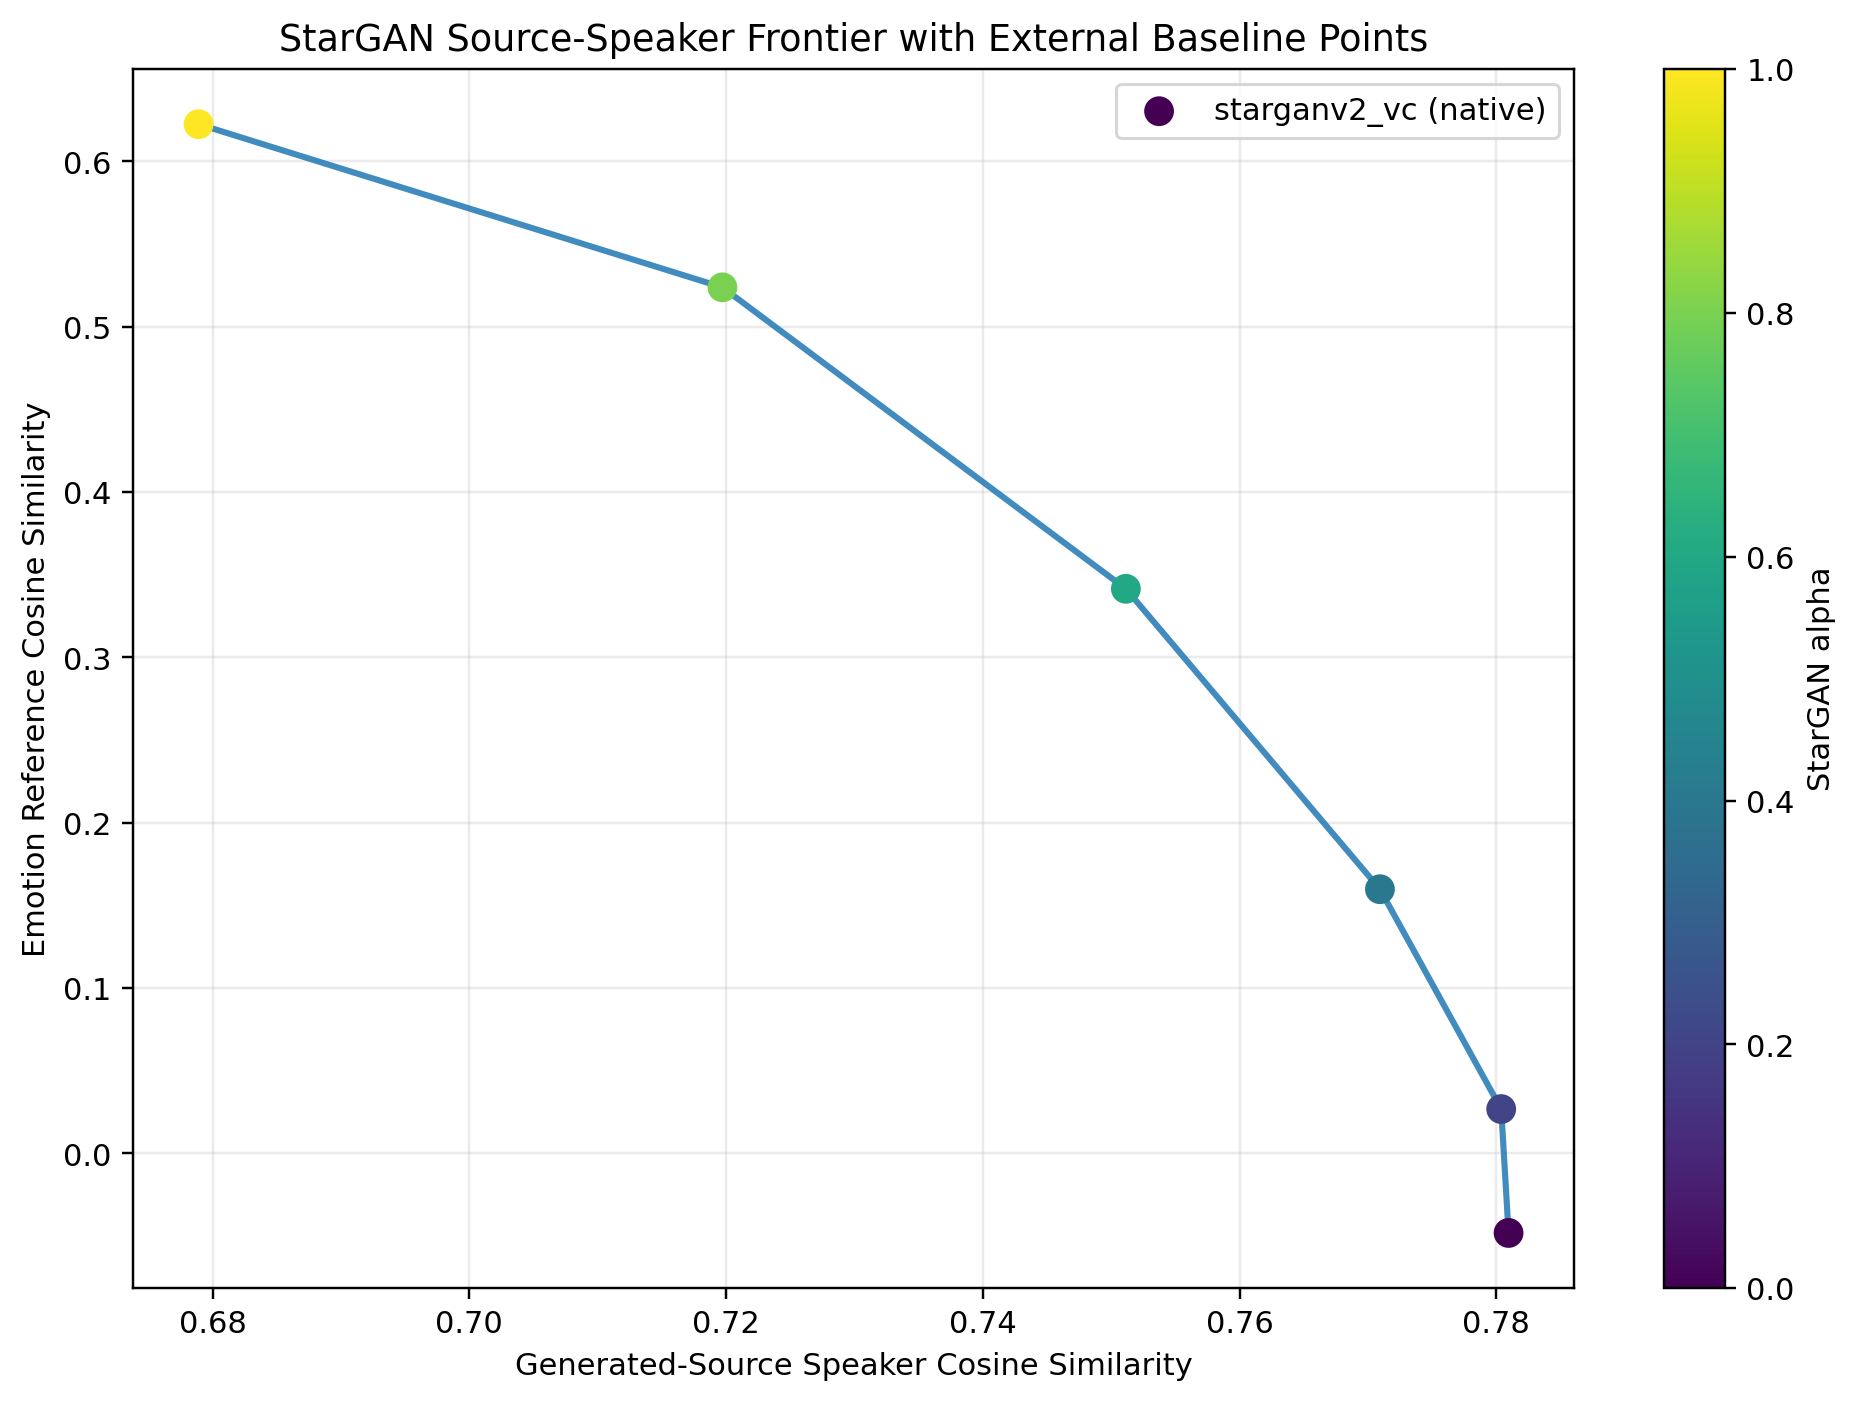
\includegraphics[width=\linewidth]{figures/frontier_native_esd_ssst.png}\\
\small (a) ESD SSST
\end{minipage}\hfill
\begin{minipage}{0.48\textwidth}
\centering
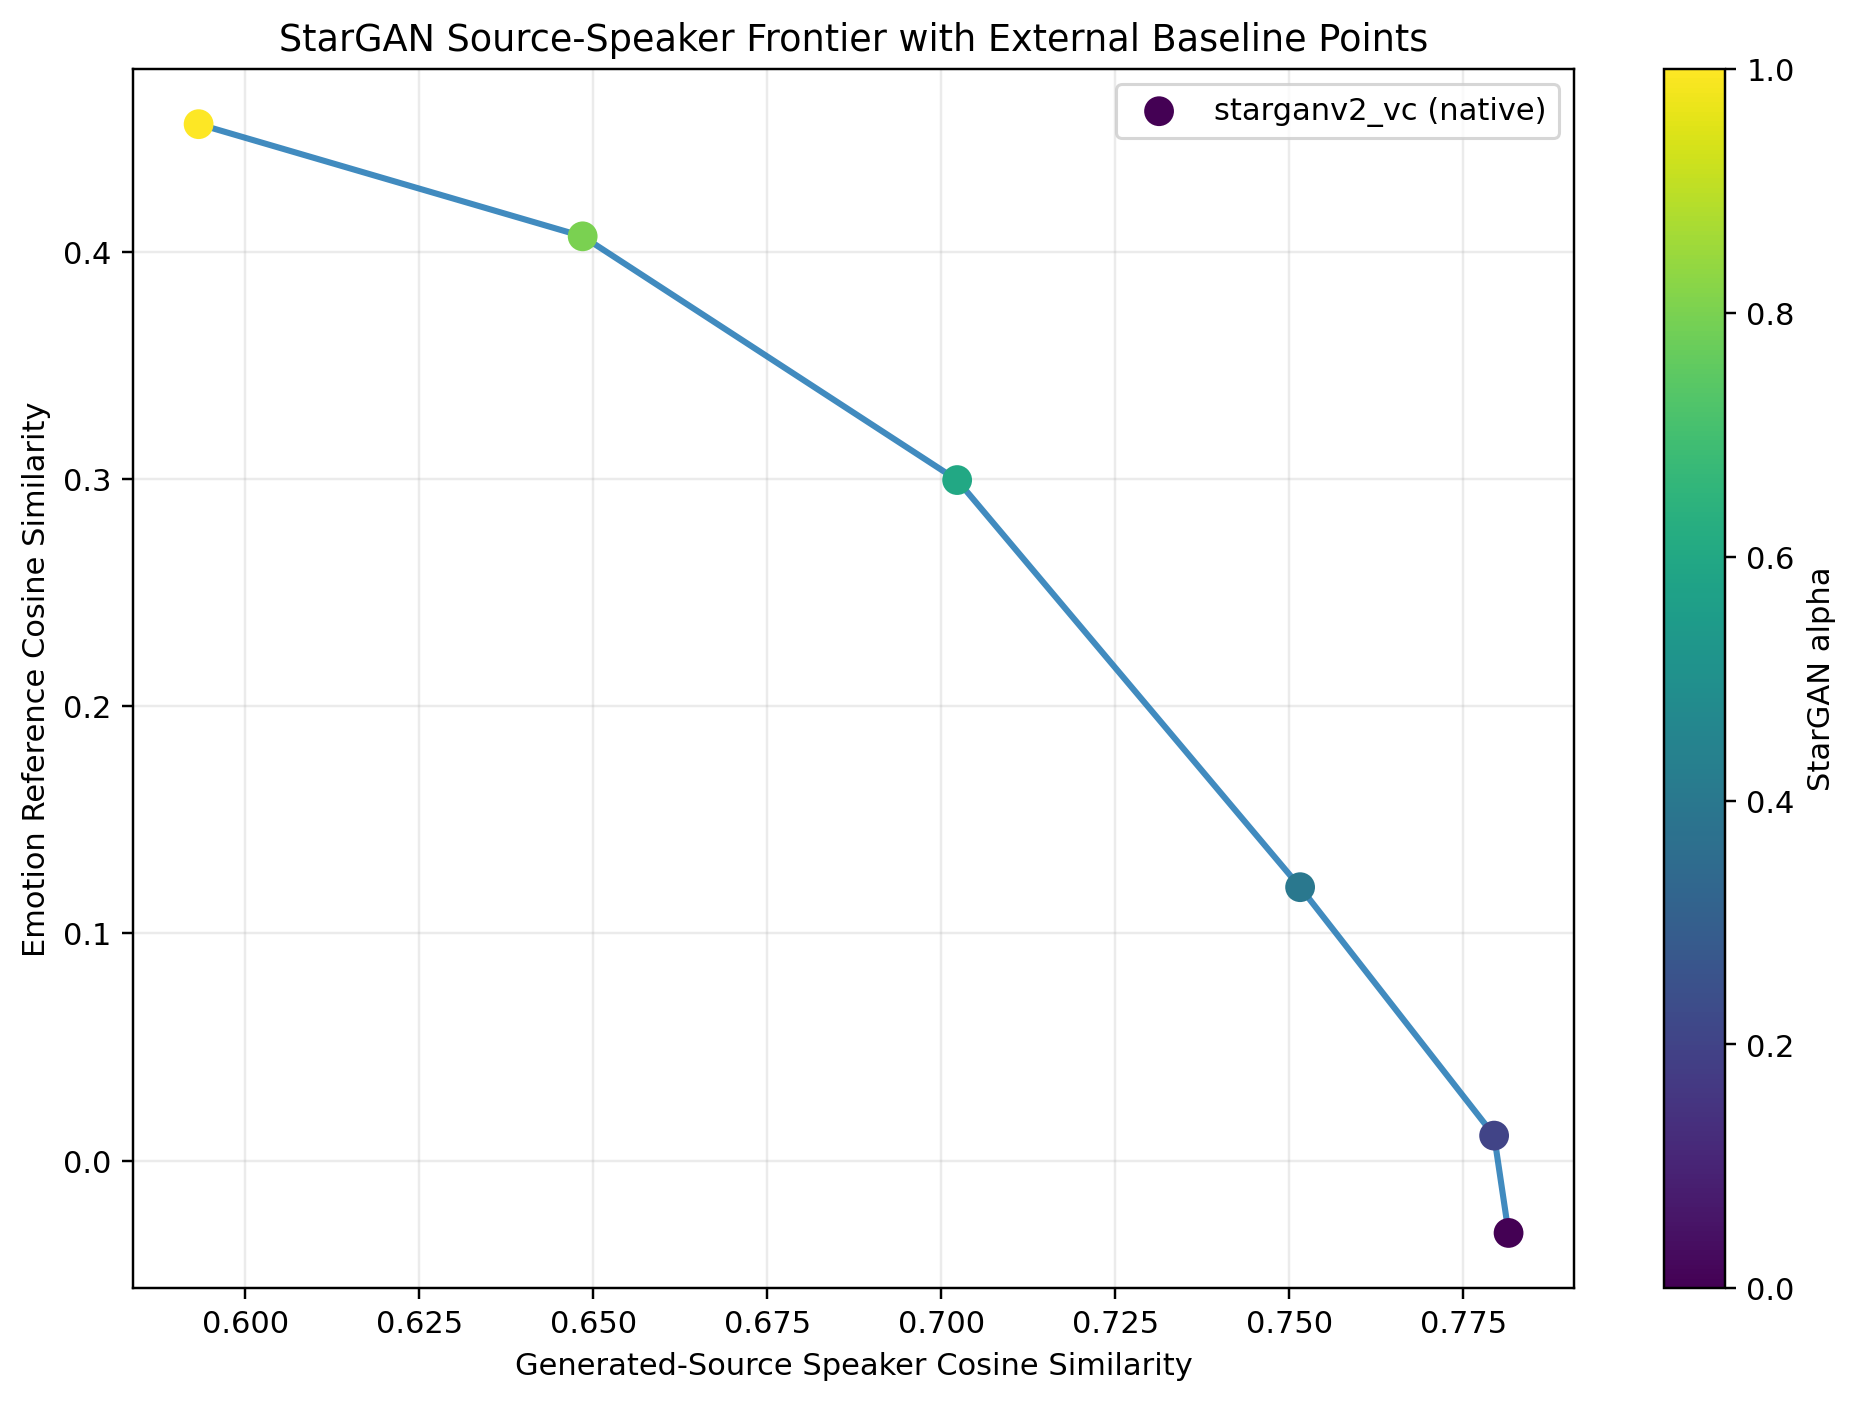
\includegraphics[width=\linewidth]{figures/frontier_native_esd_dsst.png}\\
\small (b) ESD DSST
\end{minipage}
\caption{Native-intensity source-speaker frontiers on ESD. Increasing alpha strengthens target-emotion alignment but reduces generated-source speaker similarity, with a larger speaker-preservation cost in DSST than in SSST.}
\label{fig:endpoint-tradeoff}
\end{figure*}

\begin{table*}[t]
\caption{Overall objective evaluation metrics for the propsed baselines, for each metric we record $\alpha=0$, $\alpha=1$, and $\Delta =\alpha_1-\alpha_0$. Emotion-side metrics show clear improvements with increasing $\alpha$, while speaker-side metrics show a consistent drop, especially in the DSST setting.}
\label{tab:endpoint-summary}
\centering
\tiny
\resizebox{\textwidth}{!}{%
\begin{tabular}{ll*{12}{r}}
\toprule
Model & Dataset &
\multicolumn{3}{c}{$\mathrm{ACC}_{\mathrm{emo}}$} &
\multicolumn{3}{c}{$\mathrm{CONF}_{\mathrm{emo}}$} &
\multicolumn{3}{c}{$\mathrm{SIM}_{\mathrm{emo}}$} &
\multicolumn{3}{c}{$\mathrm{SIM}_{\mathrm{spk-src}}$} \\
\cmidrule(lr){3-5}\cmidrule(lr){6-8}\cmidrule(lr){9-11}\cmidrule(lr){12-14}
 & & $\alpha_0$ & $\alpha_1$ & $\Delta$ & $\alpha_0$ & $\alpha_1$ & $\Delta$ & $\alpha_0$ & $\alpha_1$ & $\Delta$ & $\alpha_0$ & $\alpha_1$ & $\Delta$ \\
\midrule
StarGANv2-IEVC  & ESD SSST & 0.194 & 0.664 & 0.470 & 0.192 & 0.660 & 0.468 & -0.037 & 0.602 & 0.639 & 0.780 & 0.683 & -0.097 \\
CycleGAN-IEVC & ESD SSST & 0.208 & 0.481 & 0.274 & 0.207 & 0.482 & 0.275 & 0.012 & 0.418 & 0.406 & 0.876 & 0.730 & -0.146 \\
\\
StarGANv2-NEVC (proposed)  & ESD SSST & 0.190 & 0.654 & 0.464 & 0.191 & 0.653 & 0.462 & -0.048 & \textbf{0.623} & 0.671 & 0.781 & 0.679 & -0.102 \\
StarGANv2-NEVC w/ Speaker-Classifier & ESD SSST & 0.191 & \textbf{0.674} & 0.482 & 0.192 & \textbf{0.673} & 0.481 & -0.054 & 0.606 & 0.660 & 0.783 & 0.714 & \textbf{-0.069} \\
StarGANv2-NEVC w/ Speaker-Contrastive & ESD SSST & 0.182 & 0.506 & 0.324 & 0.183 & 0.506 & 0.323 & -0.077 & 0.429 & 0.506 & 0.821 & \textbf{0.746} & -0.075 \\
\midrule
StarGANv2-IEVC & ESD DSST & 0.201 & 0.544 & 0.343 & 0.202 & 0.545 & 0.344 & -0.021 & 0.481 & 0.502 & 0.783 & 0.592 & -0.191 \\
CycleGAN-IEVC & ESD DSST & 0.058 & \textbf{0.642} & 0.583 & 0.059 & \textbf{0.640} & 0.581 & -0.156 & \textbf{0.500} & 0.656 & 1.000 & 0.706 & -0.294 \\
\\
StarGANv2-NEVC & ESD DSST & 0.190 & 0.515 & 0.325 & 0.191 & 0.514 & 0.323 & -0.032 & 0.456 & 0.488 & 0.782 & 0.593 & -0.188 \\
StarGANv2-NEVC w/ Speaker-Classifier & ESD DSST & 0.215 & 0.552 & 0.337 & 0.215 & 0.550 & 0.335 & -0.019 & 0.470 & 0.489 & 0.783 & 0.673 & -0.110 \\
StarGANv2-NEVC w/ Speaker-Contrastive & ESD DSST & 0.220 & 0.388 & 0.168 & 0.218 & 0.382 & 0.163 & -0.021 & 0.321 & 0.342 & 0.822 & \textbf{0.746} & \textbf{-0.076} \\
\midrule
StarGANv2-IEVC & CREMA-D & 0.280 & 0.259 & -0.021 & 0.278 & 0.258 & -0.019 & 0.291 & 0.318 & 0.027 & 0.302 & 0.302 & 0.000 \\
CycleGAN-IEVC & CREMA-D & 0.304 & \textbf{0.553} & 0.249 & 0.304 & \textbf{0.549} & 0.245 & 0.323 & 0.426 & 0.103 & 0.719 & 0.392 & -0.327 \\
\\
StarGANv2-NEVC w/ Speaker-Classifier & CREMA-D & 0.336 & 0.457 & 0.121 & 0.334 & 0.454 & 0.120 & 0.308 & \textbf{0.471} & 0.163 & 0.460 & \textbf{0.461} & \textbf{0.001} \\

\bottomrule
\end{tabular}
}
\end{table*}

Figure~\ref{fig:endpoint-tradeoff} and Table~\ref{tab:endpoint-summary} show the general frontier pattern.
Across ESD SSST, both StarGANv2-IEVC and StarGANv2-NEVC increase target-emotion scores as alpha moves from 0 to 1, but both lose source-speaker similarity.
StarGANv2-IEVC raises $\mathrm{ACC}_{\mathrm{emo}}$ from 0.194 to 0.664 and $\mathrm{SIM}_{\mathrm{emo}}$ from -0.037 to 0.602, while $\mathrm{SIM}_{\mathrm{spk-src}}$ drops from 0.780 to 0.683.
StarGANv2-NEVC follows the same frontier direction, with $\mathrm{ACC}_{\mathrm{emo}}$ rising from 0.190 to 0.654 and $\mathrm{SIM}_{\mathrm{spk-src}}$ falling from 0.781 to 0.679.
The speaker-classifier branch gives the best SSST alpha-1 target-class score and the smallest SSST speaker delta, but its emotion-reference cosine is lower than the proposed NEVC row.

The DSST setting makes the tradeoff more severe and exposes stronger model differences.
CycleGAN-IEVC has the largest alpha-1 emotion scores on DSST, reaching 0.642 $\mathrm{ACC}_{\mathrm{emo}}$, but it also has the largest speaker drop, -0.294.
The contrastive NEVC branch has the strongest DSST speaker preservation at alpha 1, 0.746, and the smallest absolute speaker delta, -0.076, but its emotion accuracy is only 0.388.
This is the clearest table-level evidence for the core claim: the model that looks best by target emotion is not the model that best preserves source-speaker identity.
Thus the relevant result is not a single endpoint, but the shape and location of the emotion--speaker operating point.

\subsection{Per-Dataset Evidence}

\begin{figure*}[t]
\centering
\begin{minipage}{0.48\textwidth}
\centering
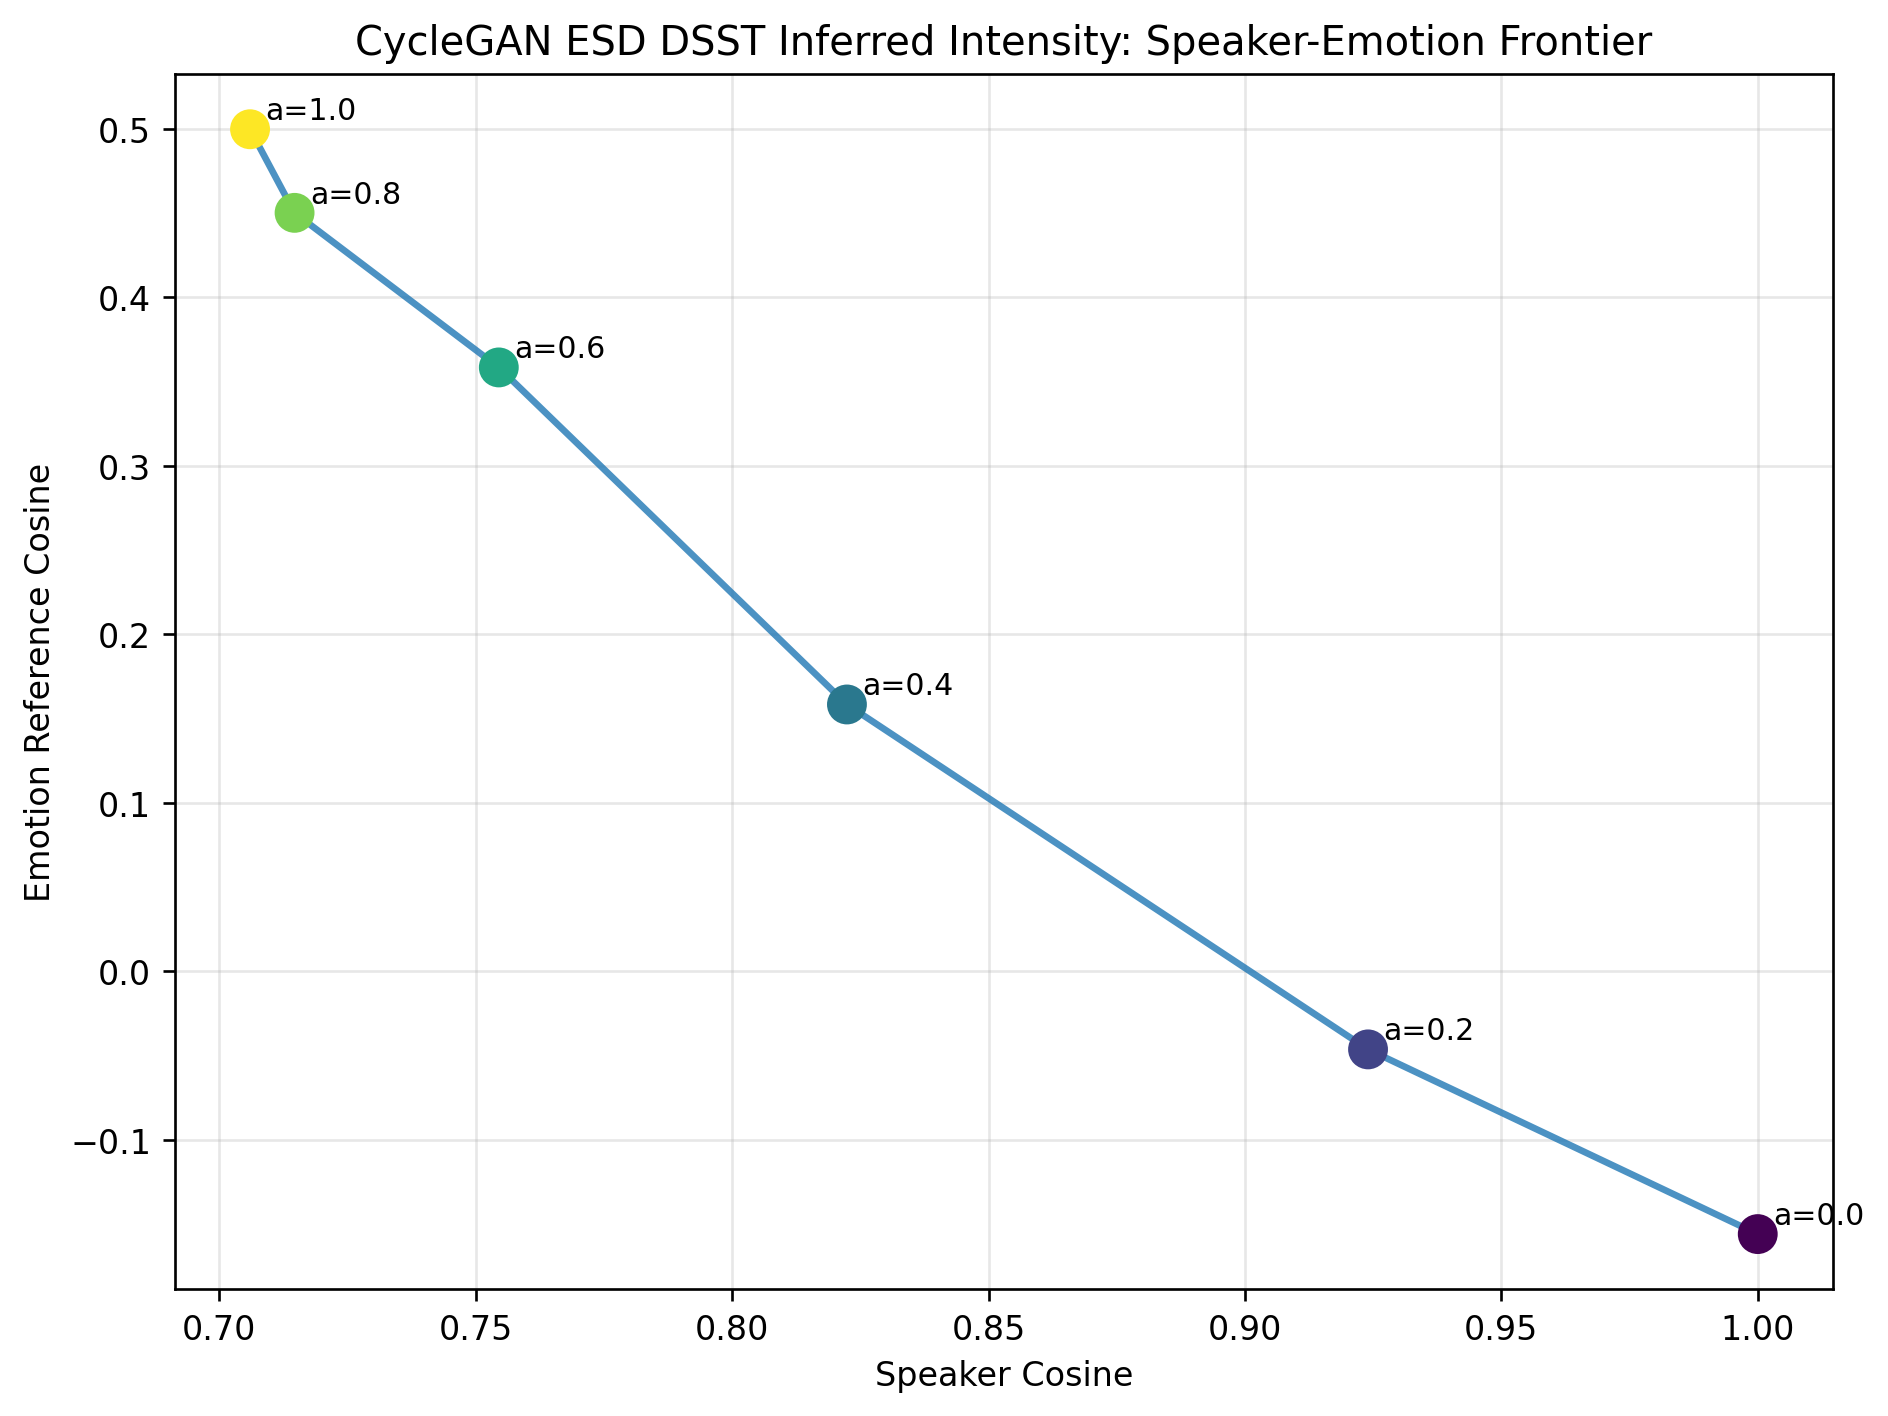
\includegraphics[width=\linewidth]{figures/frontier_cyclegan_esd_dsst.png}\\
\small (a) CycleGAN, ESD DSST
\end{minipage}\hfill
\begin{minipage}{0.48\textwidth}
\centering
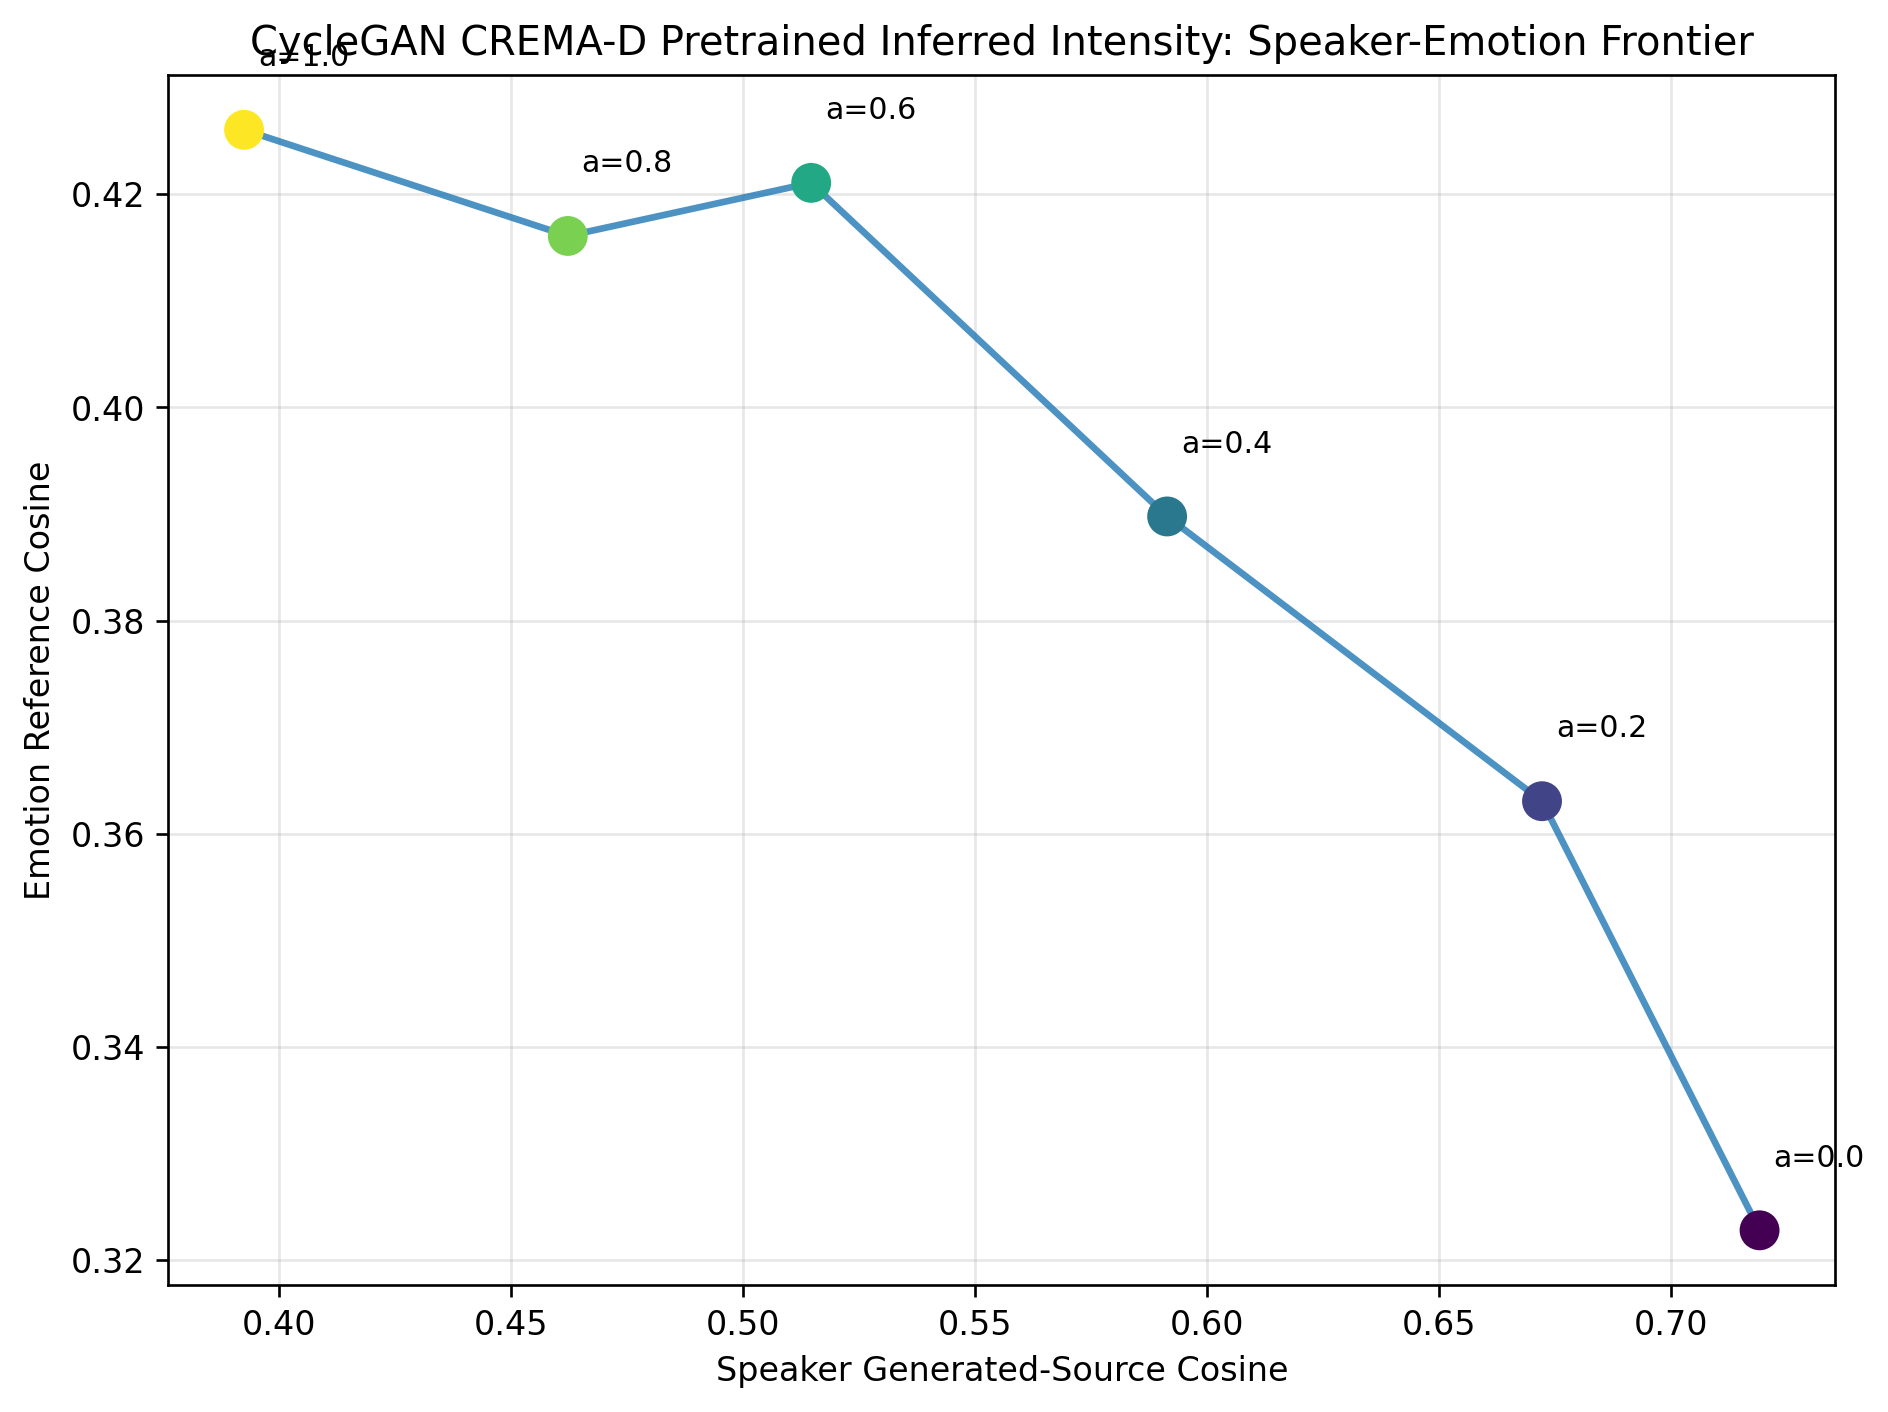
\includegraphics[width=\linewidth]{figures/frontier_cyclegan_cremad_from_scratch.png}\\
\small (b) CycleGAN, CREMA-D from scratch
\end{minipage}
\caption{CycleGAN spectrum-conversion frontiers. CycleGAN reaches strong target-emotion endpoints, but the curves occupy a higher-drift region than the StarGAN-style intensity sweeps.}
\label{fig:cyclegan-frontier}
\end{figure*}

\begin{figure*}[t]
\centering
\begin{minipage}{0.48\textwidth}
\centering
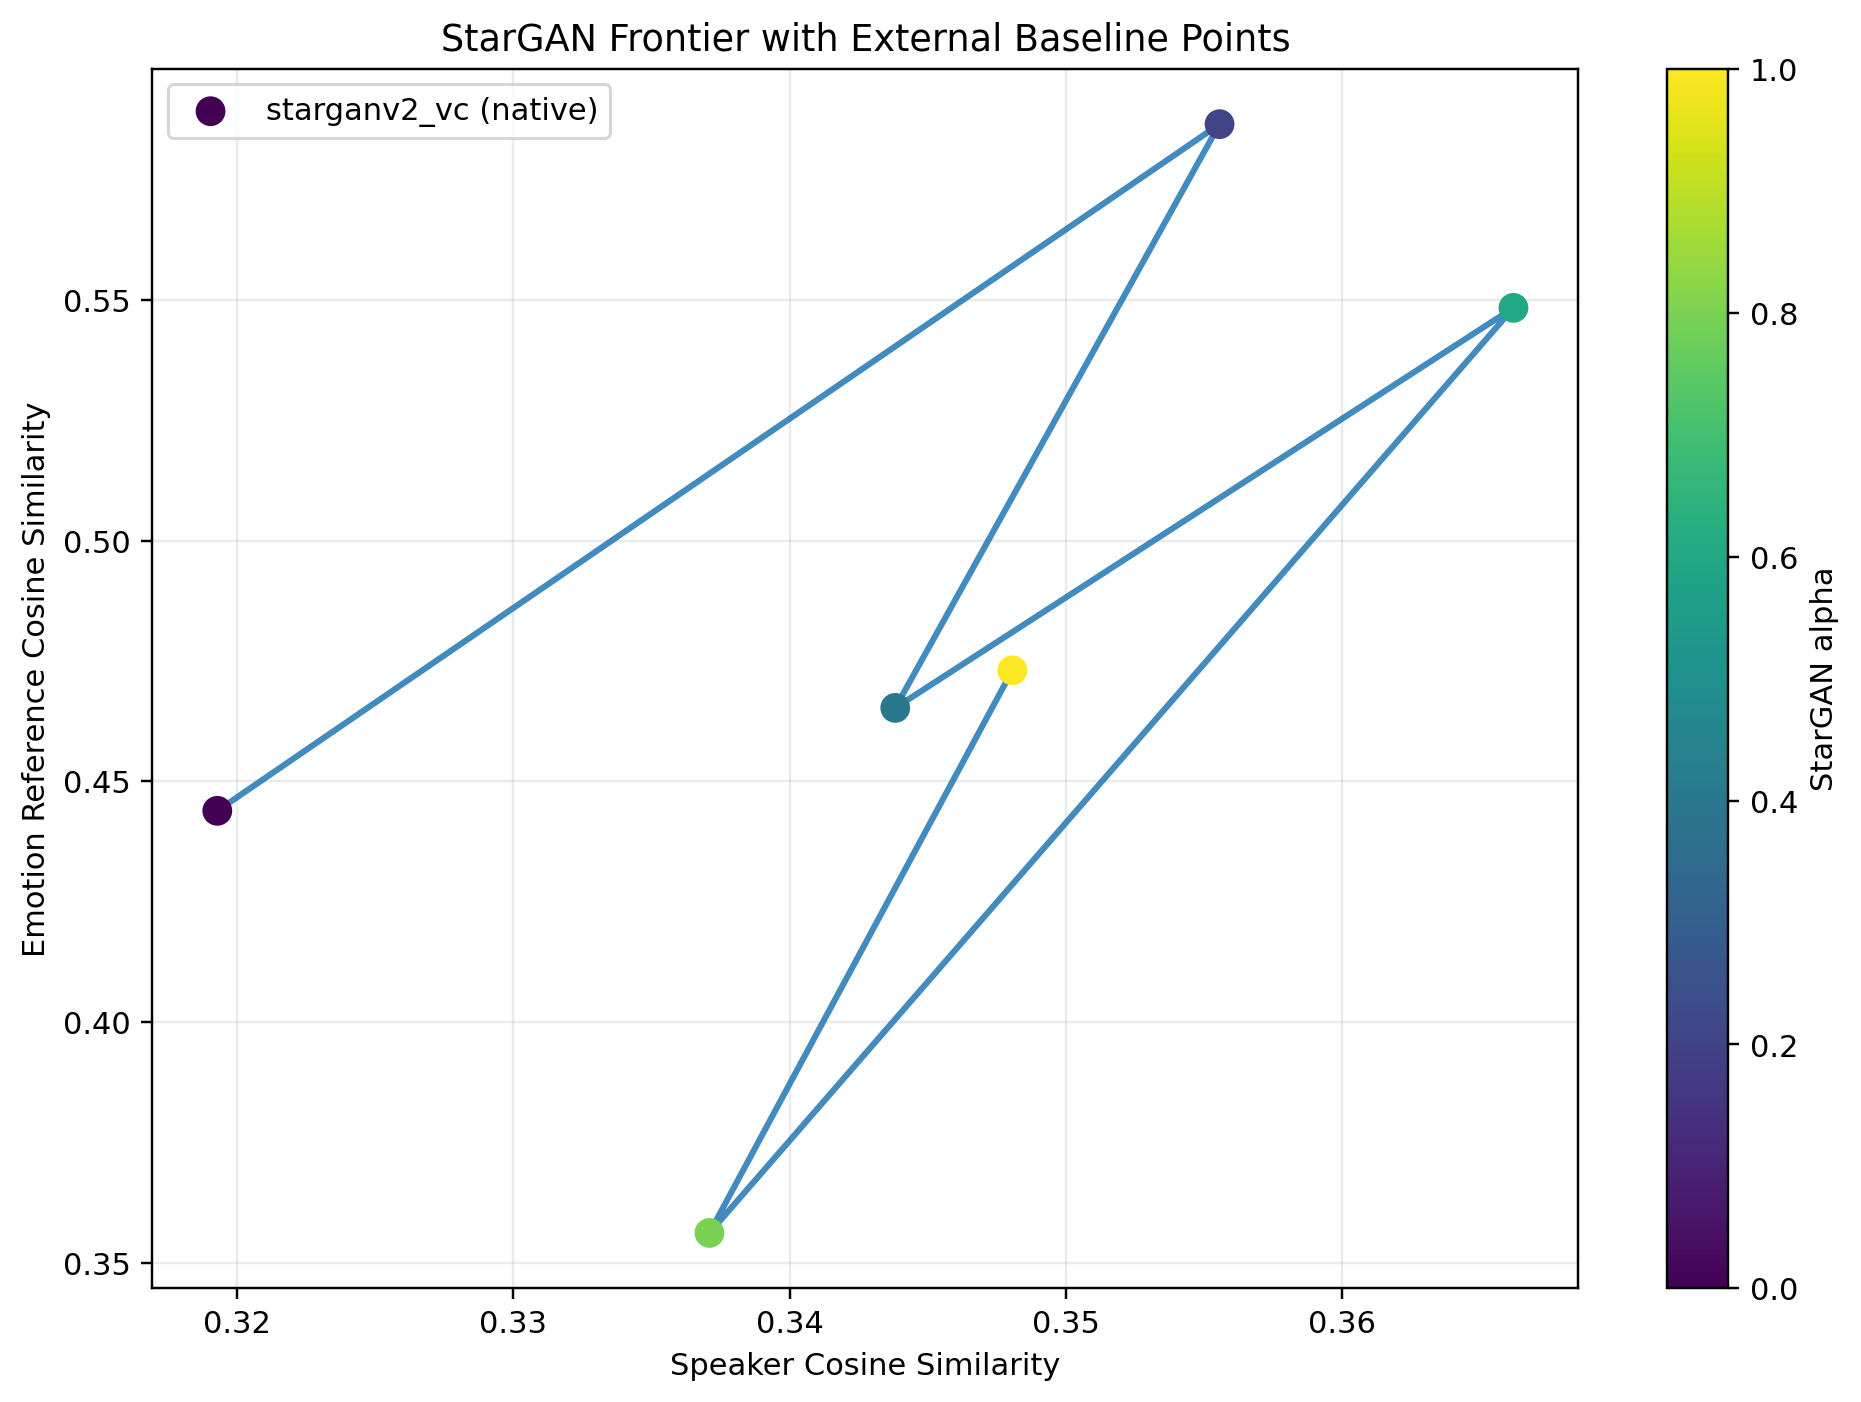
\includegraphics[width=\linewidth]{figures/frontier_native_cremad_from_scratch_epoch30.png}\\
\small (a) Native ranker, epoch 30
\end{minipage}\hfill
\begin{minipage}{0.48\textwidth}
\centering
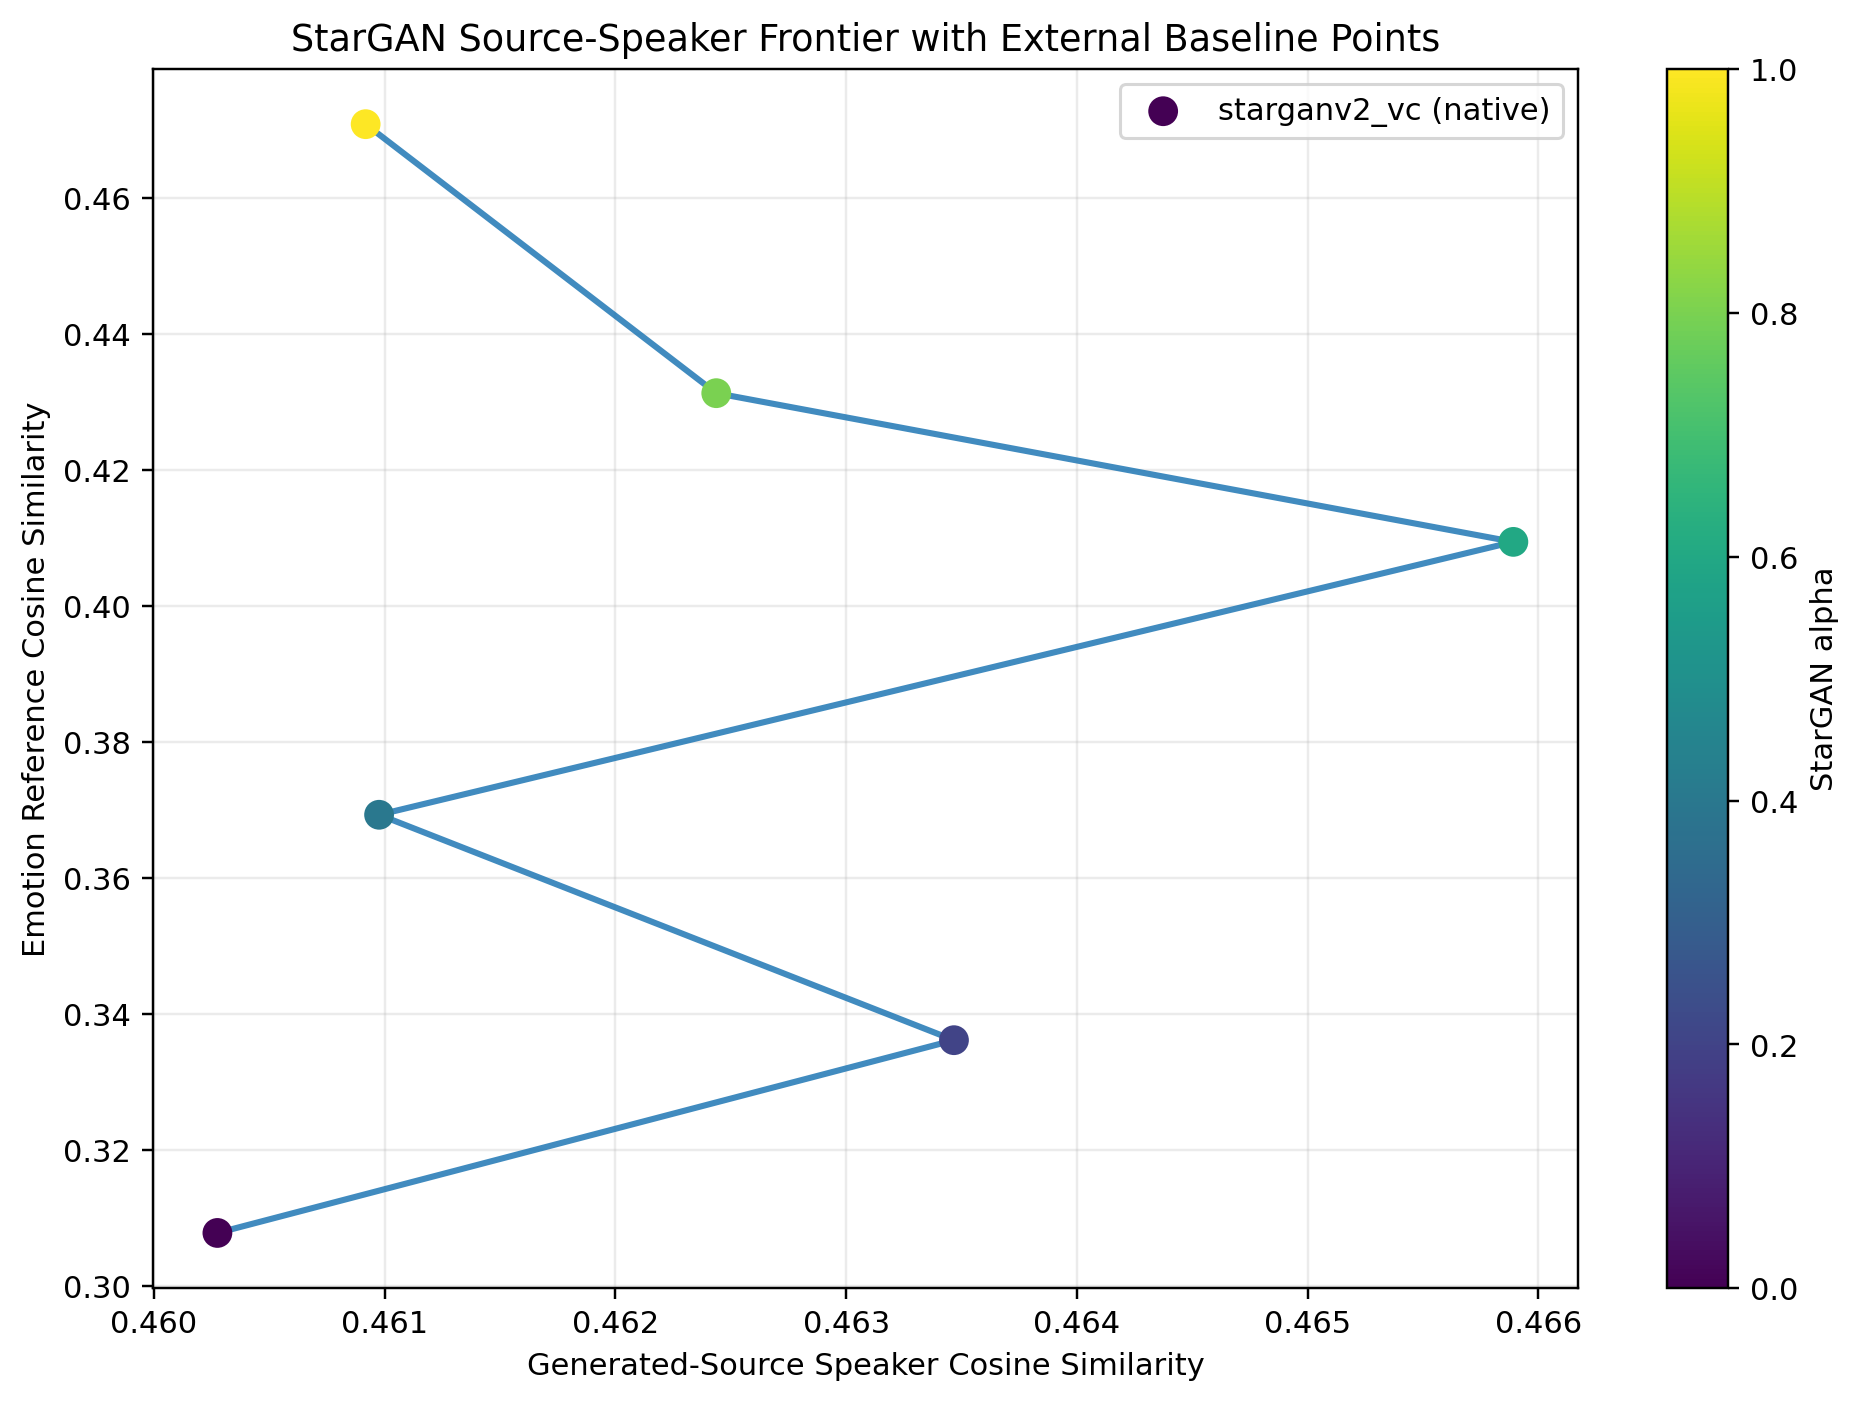
\includegraphics[width=\linewidth]{figures/frontier_ablation_speaker_cls_cremad_from_scratch.png}\\
\small (b) Speaker-classifier branch
\end{minipage}
\caption{CREMA-D from-scratch frontiers. The from-scratch condition is a stress test: the native ranker is unstable and emotion-specific, while the speaker-classifier branch is the strongest StarGAN-style from-scratch condition.}
\label{fig:cremad-from-scratch}
\end{figure*}

The dataset-level evidence has two different roles.
ESD is the main frontier evidence because both SSST and DSST produce structured alpha curves with clear emotion gains and measurable speaker losses.
CREMA-D from scratch is not a clean replication of the ESD pattern; it is a stress test for whether the same evaluation exposes unstable or dataset-dependent behavior.
In Table~\ref{tab:endpoint-summary}, CycleGAN-IEVC reaches the highest CREMA-D emotion accuracy at alpha 1, 0.553, but its source-speaker cosine falls sharply from 0.719 to 0.392.
By contrast, the speaker-classifier StarGANv2-NEVC row reaches lower alpha-1 accuracy, 0.457, but has the best CREMA-D source-speaker cosine at alpha 1, 0.461, and almost no speaker delta.

Figure~\ref{fig:cyclegan-frontier} shows why CycleGAN is useful as a baseline.
It occupies high-emotion, high-drift regions: this is especially visible on DSST and CREMA-D, where emotion scores can be strong while source-speaker preservation degrades substantially.
Figure~\ref{fig:cremad-from-scratch} shows the complementary StarGAN-style result.
The speaker-classifier branch is the more stable CREMA-D from-scratch operating point, improving emotion-reference similarity while keeping source-speaker cosine nearly unchanged.
The conclusion is therefore bounded: CREMA-D does not prove a universal frontier shape, but it shows that the proposed evaluation can distinguish high-emotion/high-drift systems from more speaker-stable operating points.

\subsection{Per-Emotion Evidence}

\begin{figure}[t]
\centering
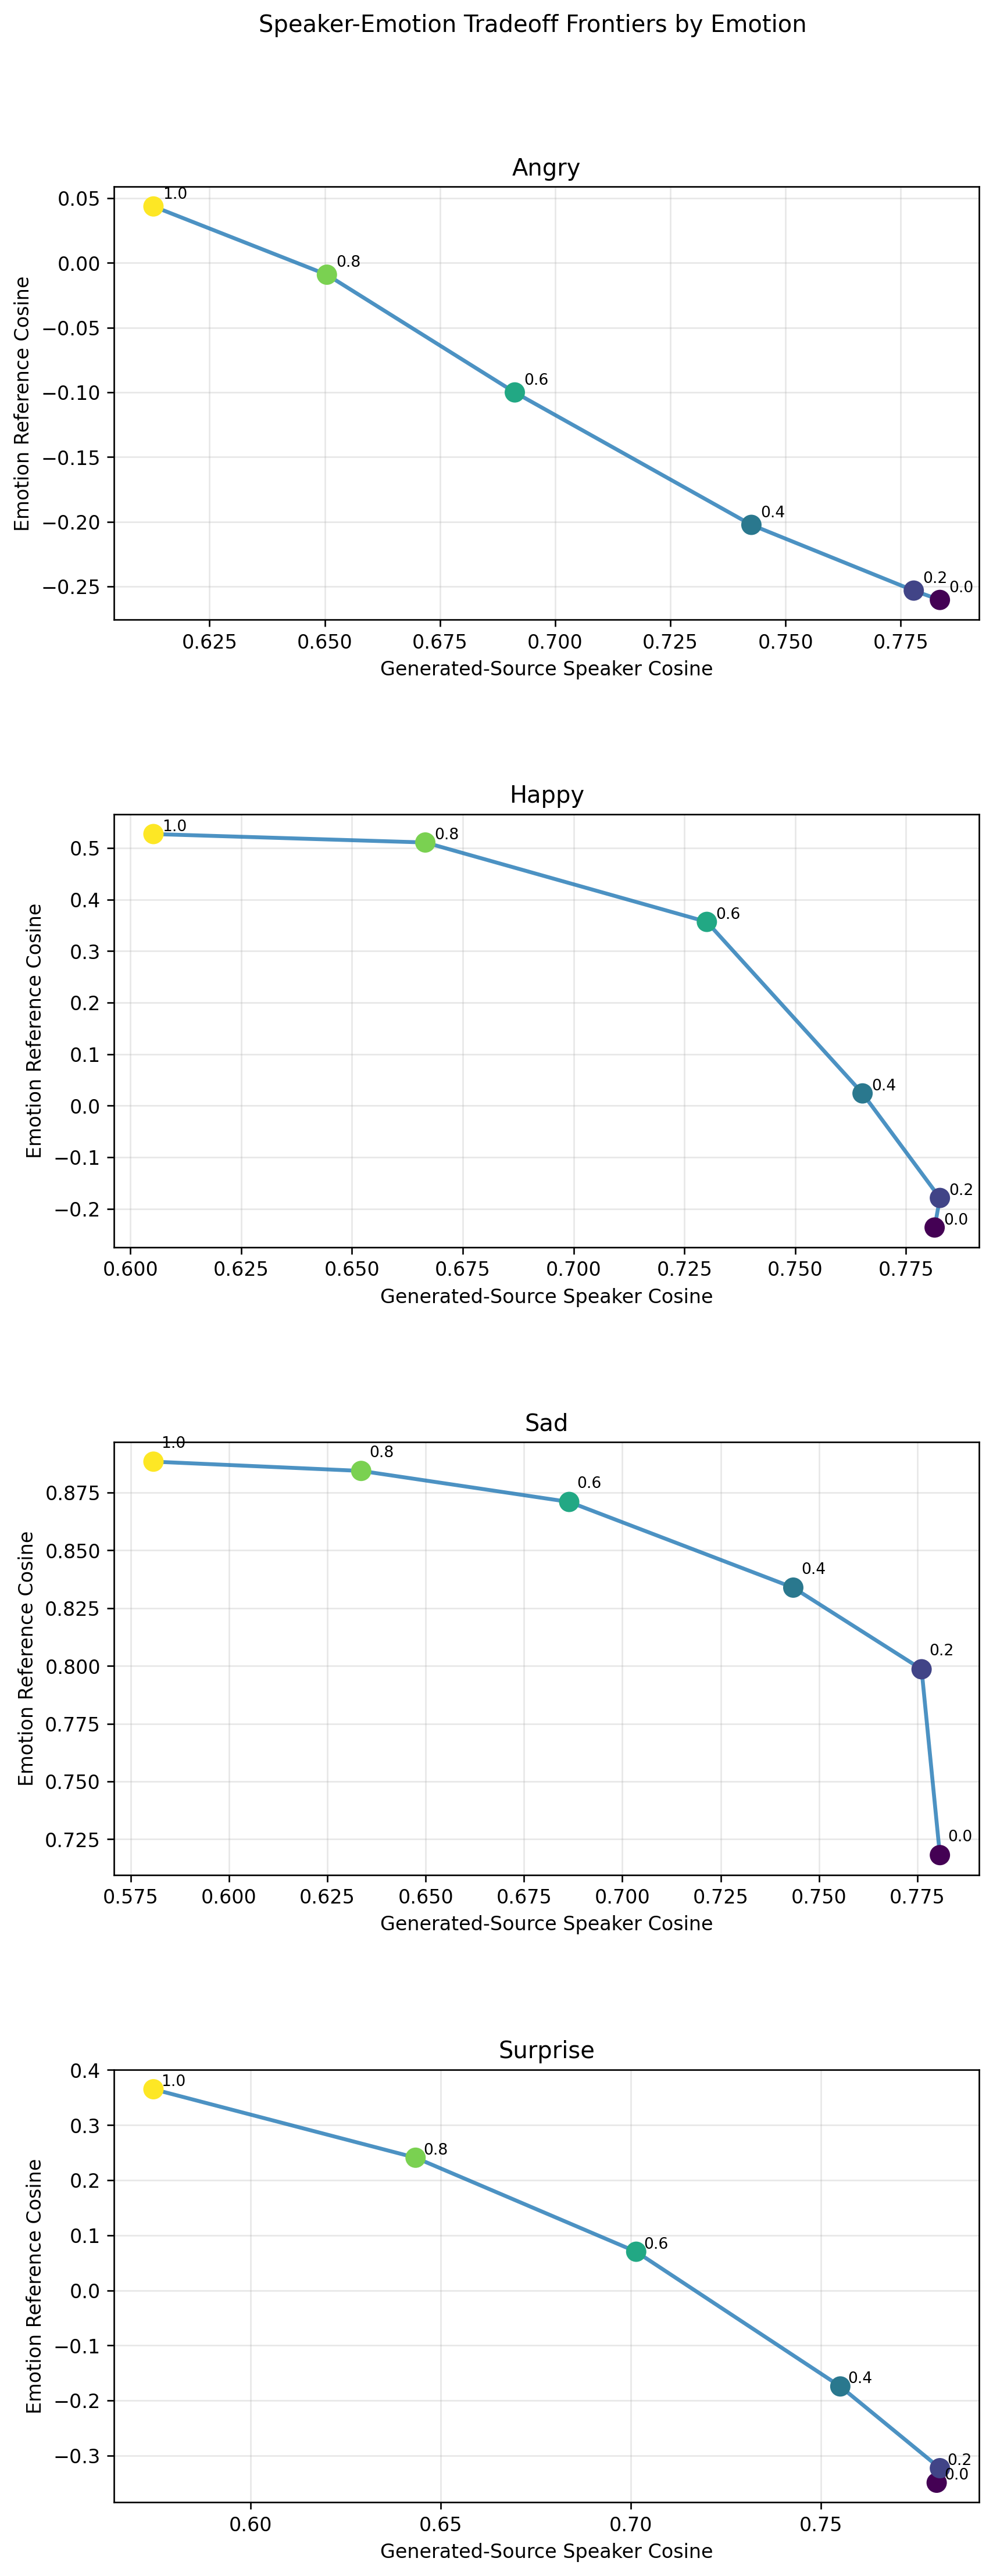
\includegraphics[height=0.82\textheight]{figures/frontier_per_emotion_native_esd_dsst.png}
\caption{Per-emotion native-intensity frontiers on ESD DSST. Sad reaches high target-emotion accuracy with a stable curve, while angry and surprise remain weak and are easy to overstate in aggregate metrics.}
\label{fig:per-emotion-frontier}
\end{figure}

\begin{table}[t]
\caption{Alpha-1 per-emotion accuracy on ESD DSST.}
\label{tab:per-emotion-dsst}
\centering
\footnotesize
\begin{tabular}{lrrrr}
\toprule
System & Angry & Happy & Sad & Surprise \\
\midrule
StarGANv2-IEVC & 0.167 & 0.652 & 0.996 & 0.359 \\
StarGANv2-NEVC & 0.163 & 0.685 & 0.996 & 0.215 \\
StarGANv2-NEVC-Spk-Cls & 0.244 & 0.652 & 0.996 & 0.315 \\
StarGANv2-NEVC-Spk-Con  & 0.040 & 0.468 & 1.000 & 0.033 \\
\bottomrule
\end{tabular}
\end{table}

Figure~\ref{fig:per-emotion-frontier} and Table~\ref{tab:per-emotion-dsst} show that aggregate curves hide large label differences.
For native intensity on ESD DSST, sad reaches 0.996 accuracy and happy reaches 0.685, but angry and surprise remain much weaker at 0.163 and 0.215.
The speaker-classifier branch improves the weak labels somewhat, reaching 0.244 for angry and 0.315 for surprise, while keeping sad at 0.996.
The contrastive branch exposes the opposite failure mode: it preserves speakers well but collapses difficult emotion transfer, with angry and surprise falling to 0.040 and 0.033.
The conclusion is that the tradeoff is not uniform across emotions; per-emotion plots are necessary to prevent sad-dominated aggregate scores from overstating controllability.

\subsection{Model Comparisons and Significance}

\begin{figure*}[t]
\centering
\begin{minipage}{0.48\textwidth}
\centering
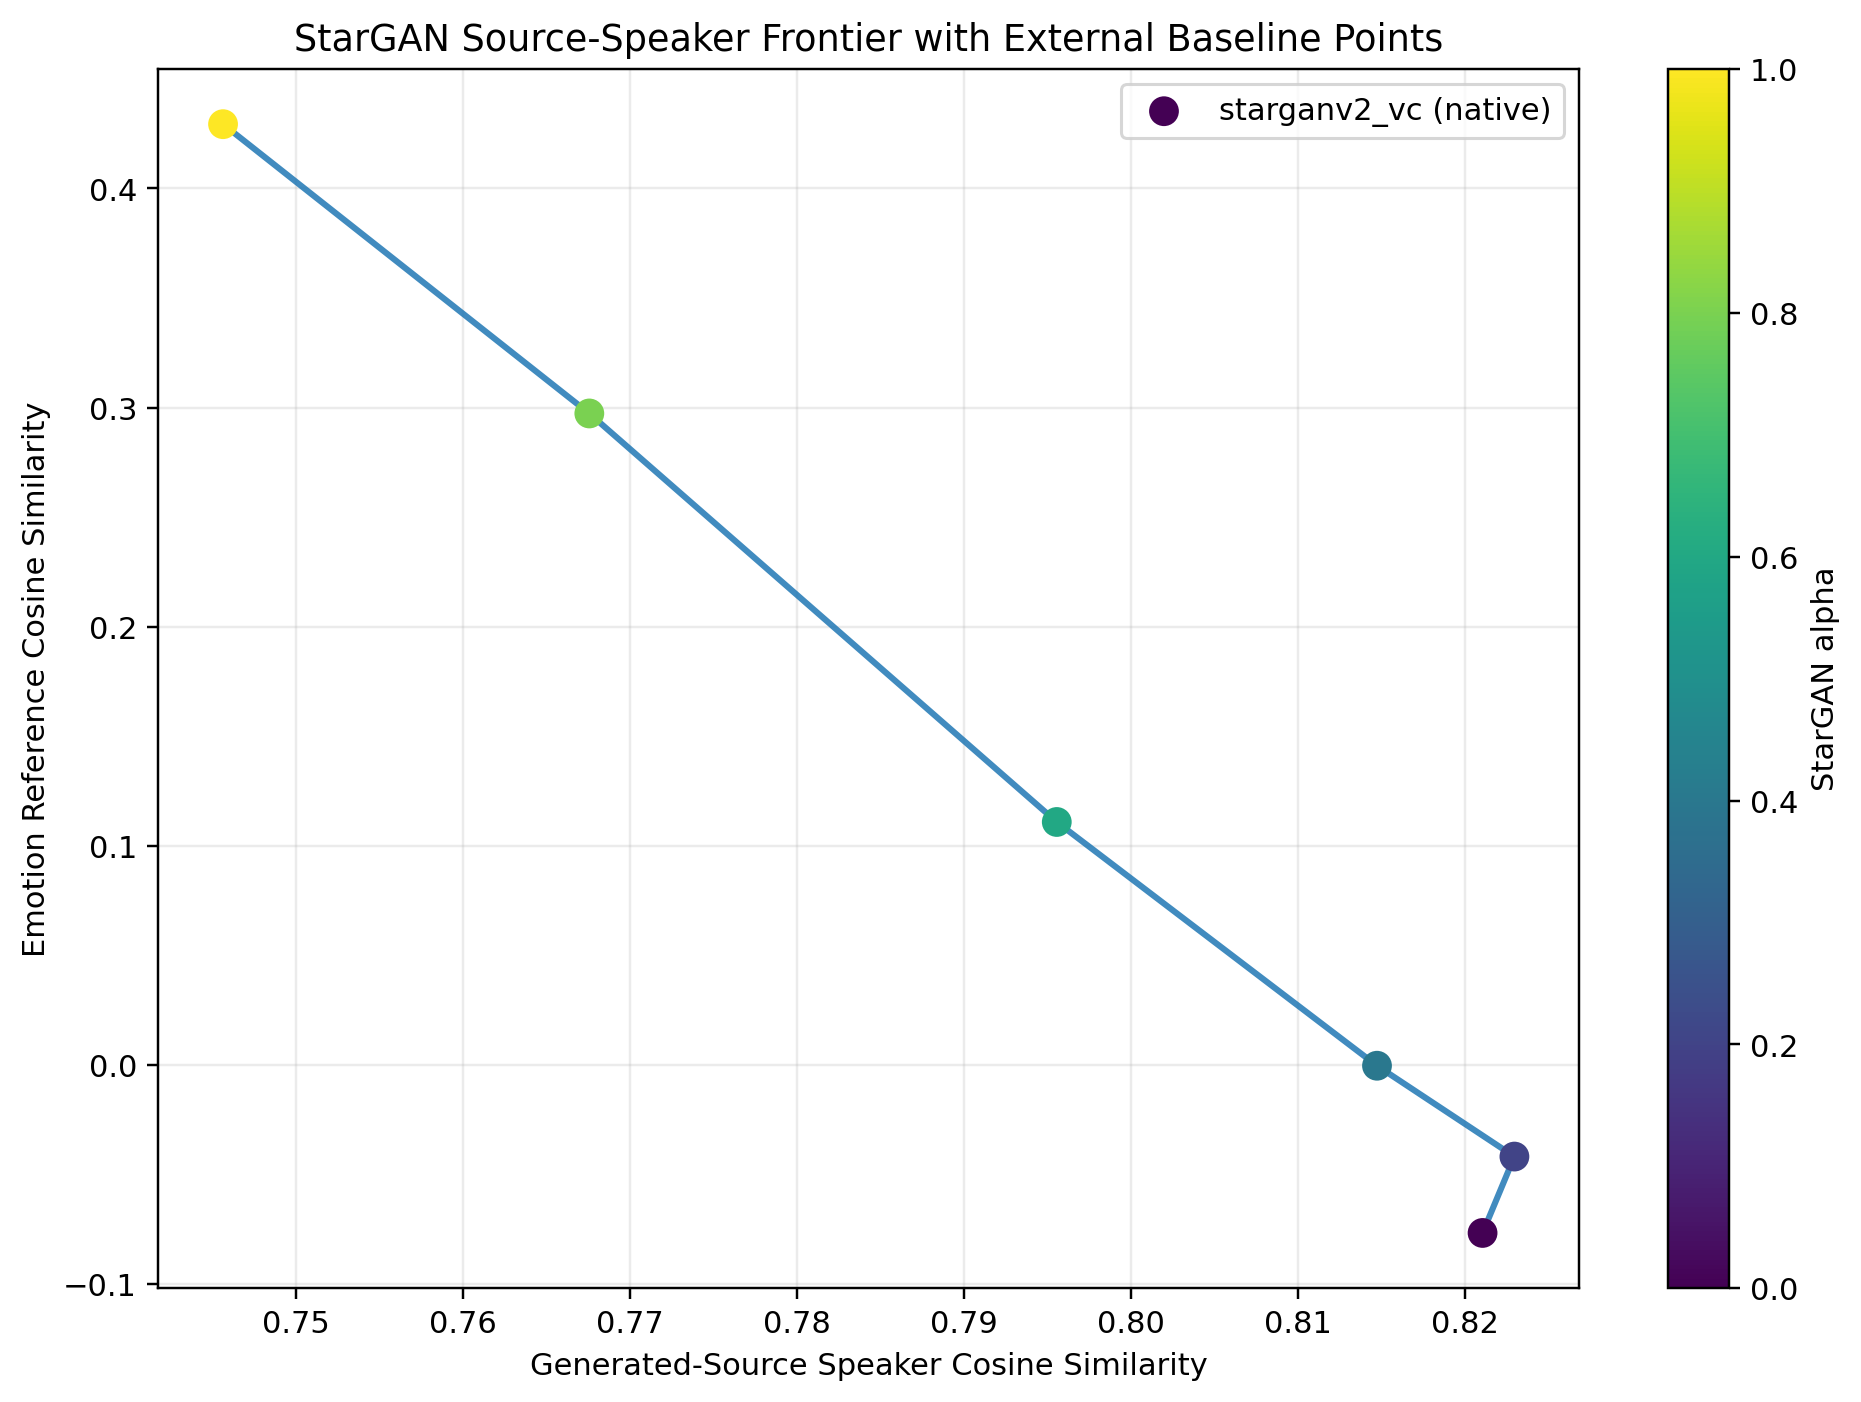
\includegraphics[width=\linewidth]{figures/frontier_ablation_speaker_contrastive_esd_ssst.png}\\
\small (a) Contrastive branch, ESD SSST
\end{minipage}\hfill
\begin{minipage}{0.48\textwidth}
\centering
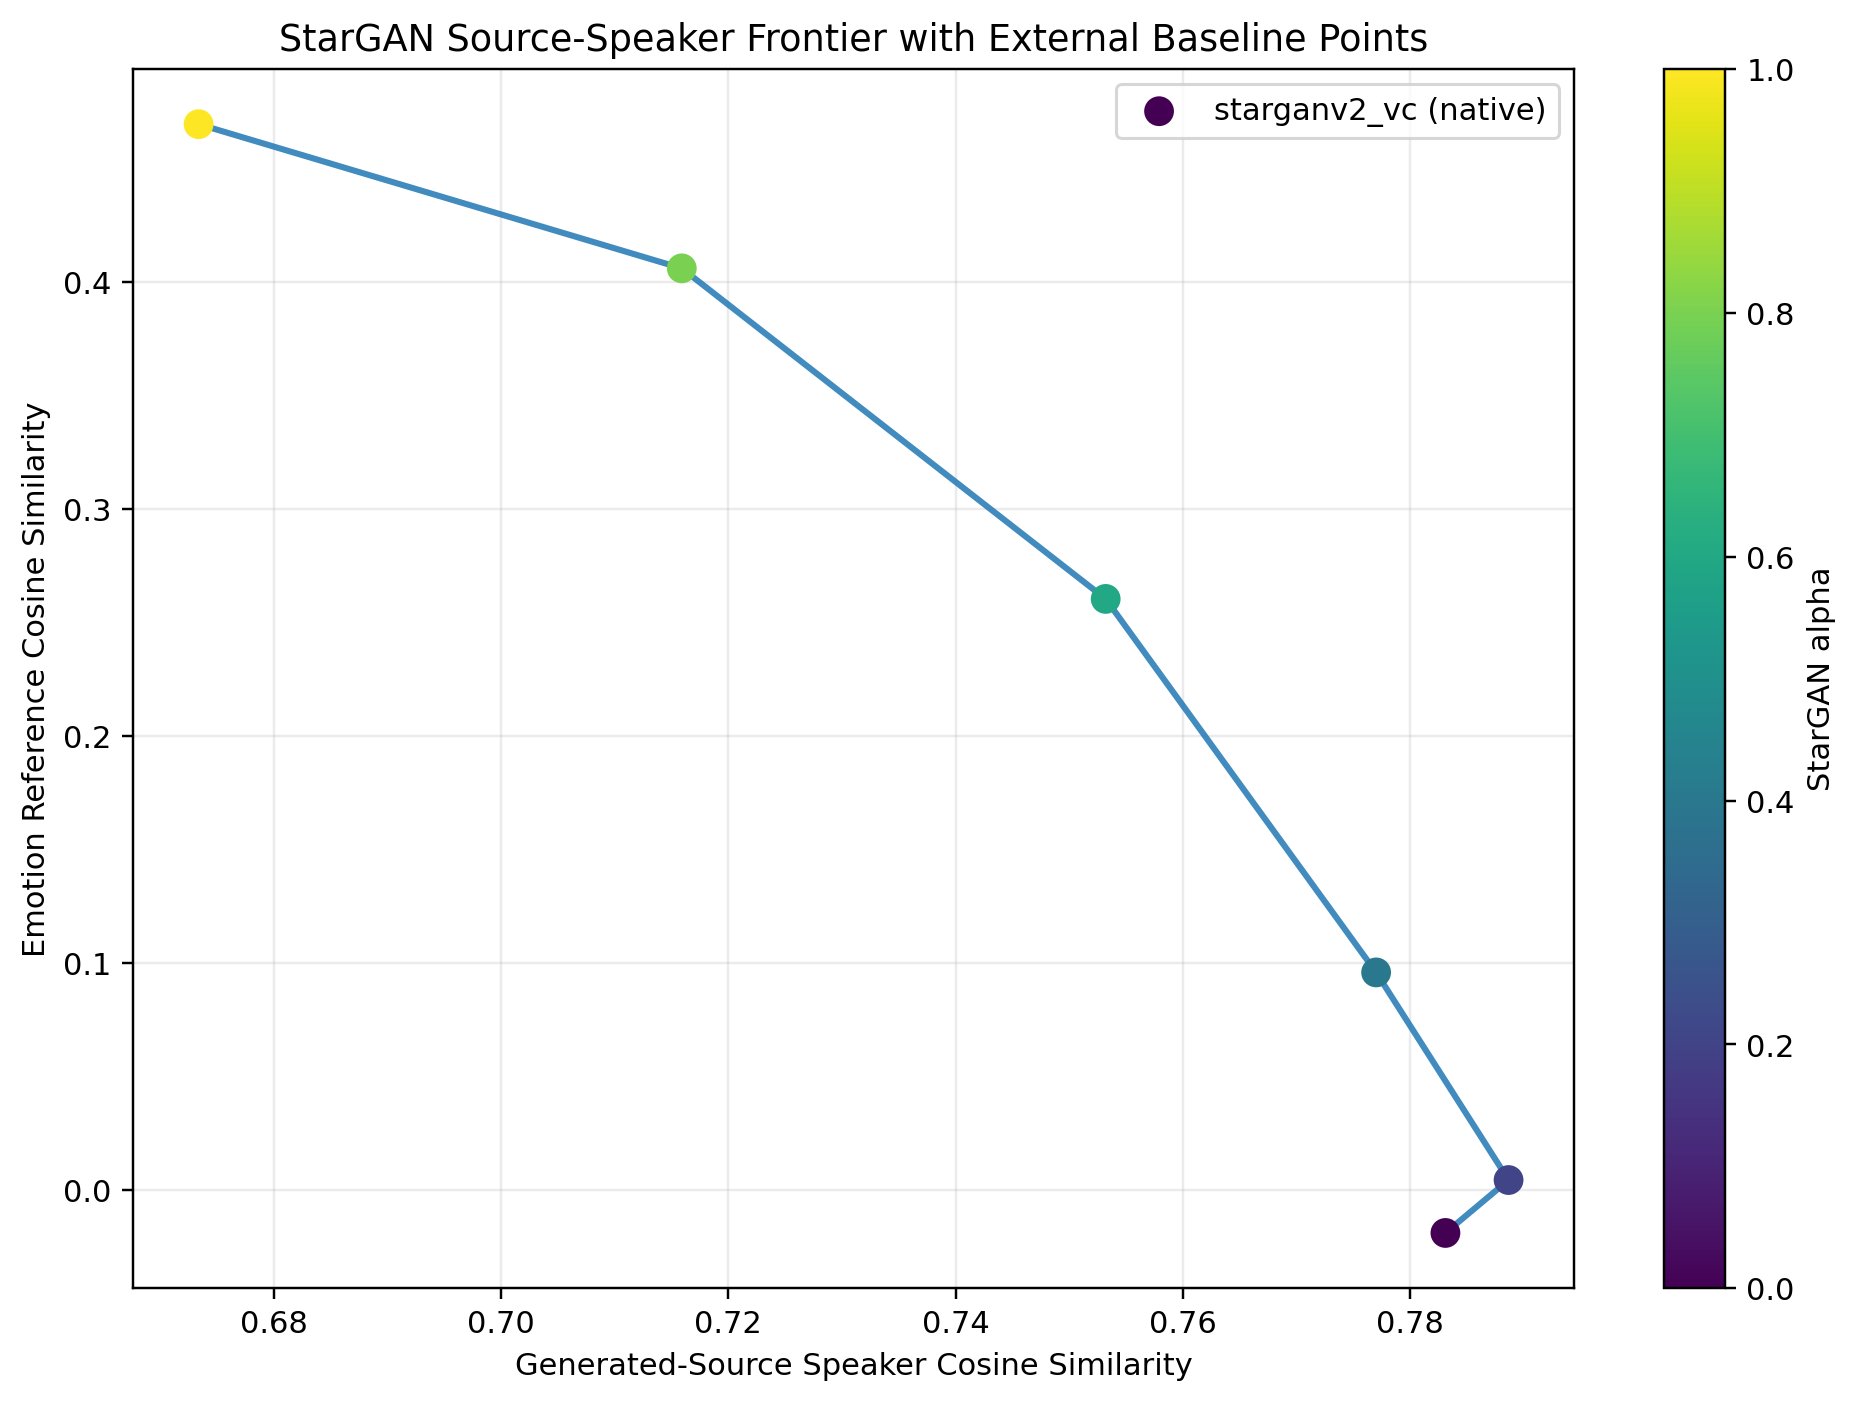
\includegraphics[width=\linewidth]{figures/frontier_ablation_speaker_cls_esd_dsst.png}\\
\small (b) Speaker-classifier branch, ESD DSST
\end{minipage}
\caption{Speaker-related ablation frontiers on ESD. The contrastive branch shifts toward speaker preservation at the cost of target-emotion transfer. The speaker-classifier branch is more favorable on DSST, but still has metric-specific tradeoffs.}
\label{fig:ablation-frontier}
\end{figure*}

\begin{table*}[t]
\caption{Selected paired significance tests for model comparisons. $\Delta$ is left model minus right model. Positive is favorable for accuracy, emotion-reference cosine, and speaker cosine; negative is favorable for MCD.}
\label{tab:significance}
\centering
\scriptsize
\begin{tabular}{llrrrrp{0.24\textwidth}}
\toprule
Setting & Comparison and metric & Left & Right & $\Delta$ & 95\% CI & Interpretation \\
\midrule
SSST & Spk-cls. vs native, speaker cosine & 0.761 & 0.747 & 0.014 & [0.013, 0.016] & Significant speaker gain; $q<10^{-66}$. \\
SSST & Spk-cls. vs native, emotion acc. & 0.405 & 0.401 & 0.004 & [-0.007, 0.014] & No significant accuracy change. \\
SSST & Spk-cls. vs native, emotion-ref. & 0.259 & 0.271 & -0.012 & [-0.022, -0.003] & Significant emotion-reference loss; $q<10^{-5}$. \\
\midrule
DSST & Spk-cls. vs native, speaker cosine & 0.749 & 0.709 & 0.039 & [0.037, 0.041] & Significant speaker gain; $q<10^{-217}$. \\
DSST & Spk-cls. vs native, emotion acc. & 0.355 & 0.345 & 0.010 & [0.002, 0.017] & Significant accuracy gain; $q=0.022$. \\
DSST & Spk-cls. vs inferred, speaker cosine & 0.749 & 0.699 & 0.049 & [0.047, 0.052] & Significant speaker gain; $q<10^{-308}$. \\
DSST & Spk-cls. vs inferred, emotion-ref. & 0.203 & 0.212 & -0.009 & [-0.019, -0.000] & Significant emotion-reference loss; $q=0.019$. \\
\midrule
CREMA-D FS & Spk-cls. vs native, speaker cosine & 0.462 & 0.309 & 0.153 & [0.150, 0.156] & Significant speaker gain; $q=0$. \\
CREMA-D FS & Spk-cls. vs native, emotion acc. & 0.389 & 0.296 & 0.093 & [0.076, 0.111] & Significant accuracy gain; $q<10^{-25}$. \\
CREMA-D FS & Spk-cls. vs inferred, emotion-ref. & 0.388 & 0.318 & 0.070 & [0.051, 0.088] & Significant emotion-reference gain; $q<10^{-10}$. \\
CREMA-D FS & Spk-cls. vs inferred, MCD src & 406.7 & 498.9 & -92.2 & [-93.0, -91.5] & Significant lower distortion; $q=0$. \\
\bottomrule
\end{tabular}
\end{table*}

Figure~\ref{fig:ablation-frontier} and Table~\ref{tab:significance} support three model-comparison conclusions.
First, speaker supervision is not uniformly beneficial.
On SSST, the speaker-classifier branch significantly improves speaker cosine and MCD relative to the native ranker, but emotion accuracy is statistically indistinguishable and emotion-reference cosine is significantly worse.
This matches Table~\ref{tab:endpoint-summary}: the same branch has the best SSST alpha-1 accuracy and smallest speaker delta, but not the best emotion-reference cosine.

Second, the DSST setting makes the speaker-classifier branch more favorable but still metric-specific.
It significantly improves speaker cosine over both native and inferred baselines and gives a small significant accuracy gain over the native ranker.
However, its emotion-reference cosine remains worse than inferred intensity, so the result should be stated as a speaker-preservation and target-class gain, not as a general emotion-similarity improvement.
The contrastive branch represents the opposite choice: it has the best DSST speaker preservation in Table~\ref{tab:endpoint-summary}, but weak target-emotion transfer.

Third, in CREMA-D from scratch, the speaker-classifier branch is the strongest StarGAN-style operating point among the tested rows.
The paired tests show significant gains over native and inferred baselines on speaker cosine, emotion accuracy, emotion-reference cosine, emotion confidence, and MCD.
This justifies keeping it in the main comparison for CREMA-D from scratch, while still treating it as an ablation rather than replacing the native-ranker design.

\subsection{Perceptual Support}

\begin{table}[t]
\caption{Subjective listening-study scores for StarGANv2-NEVC on ESD SSST. Scores use a 1--5 scale. Nat. is naturalness, Emo. sim. is perceived emotion similarity, and Spk. sim. is perceived source-speaker similarity.}
\label{tab:listening-study}
\centering
\footnotesize
\resizebox{\columnwidth}{!}{%
\begin{tabular}{lrrrrrrr}
\toprule
$\alpha$ & $n$ & Nat. & Nat. std. & Emo. sim. & Emo. std. & Spk. sim. & Spk. std. \\
\midrule
0.0 & 100 & 2.79 & 1.71 & 2.07 & 1.89 & 4.04 & 1.29 \\
0.4 & 96 & 2.71 & 1.62 & 2.83 & 1.68 & 2.95 & 1.84 \\
0.8 & 98 & 2.54 & 1.63 & 3.31 & 1.36 & 1.84 & 1.85 \\
1.0 & 96 & 2.41 & 1.68 & 3.46 & 1.55 & 1.55 & 1.86 \\
\bottomrule
\end{tabular}
}
\end{table}

The available ESD SSST listening study supports the same direction as the automatic metrics.
Table~\ref{tab:listening-study} shows that perceived emotion similarity rises monotonically with alpha, from 2.07 at alpha 0 to 3.46 at alpha 1.
Over the same range, perceived speaker similarity drops from 4.04 to 1.55, and naturalness decreases from 2.79 to 2.41.
This perceptual pattern is important because it mirrors the automatic frontier: high-alpha samples are judged as more emotional but less source-speaker similar.
The conclusion remains bounded because the listening evidence covers only StarGANv2-IEVC on ESD SSST; DSST, CREMA-D, and the ablation branches still require matched listening tests with confidence intervals and significance analysis.
